% !TEX root=../index.tex

\chapter{Haar-like Features}
\label{cap:haar_features}
\emph{Definizione delle feature.
Derivazione delle feature dalle wavelet di Haar.
Immagini integrali.
Decision Stump.} 


La descrizione di un qualsiasi oggetto avviene attraverso la descrizione dei suoi attributi. La forma geometrica, le dimensioni, il peso, il colore sono solo una manciata dei possibili attributi con i quali descrivere un oggetto.
L'essere umano è dotato di 5 sensi attraverso i quali è in grado di \emph{percepire} la realtà circostante e di un'infinità di modi con cui \emph{descriverla}.

Il riconoscimento di un oggetto avviene solo in un secondo momento, attraverso l'analisi della sua descrizione, valutando gli attributi che, in quel contesto, sono più signicativi.
Nell'ambito della visione artificiale, il riconoscimento degli oggetti segue esattamente lo stesso flusso.
Gli attributi di un oggetto vengono descritti mediante l'utilizzo di \emph{feature}, ovvero dei meccanismi per misurare le varie proprietà dell'oggetto stesso.

Le immagini di profondità sono il frutto della percezione della realtà, le feature di Haar costituiscono gli attributi con i quali è possibile descrivere tali immagini.


\section{Definizione}
\label{sec:haar_def}
Le feature di Haar riescono a misurare la quantità e il verso delle variazioni di intensità tra due regioni adiacenti di una immagine.
La comune rappresentazione grafica di tali feature mette in evidenza le due regioni colorandone una bianco e l'altra di nero.
La somma delle intensità dei pixel della regione bianca a cui viene sottratta la somma delle intensità della regione nera fornisce una misura della variazione media di intensità tra le due regioni (equazione \ref{eq:haar_feature_informal}).

Di feature ne esistono di diverse forme: in figura \ref{fig:features_type} sono presenti quelle utilizzate in questo ambito, ma disponibili molte forme di feature utilizzate da altri sistemi di object detection. Non tutte sono formate solamente da \emph{due regioni adiacenti}, ma l'importante è che tutte abbiano una regione \emph{nera} ed una regione \emph{bianca}.

\begin{wrapfigure}{L}{0cm}
    \centering
    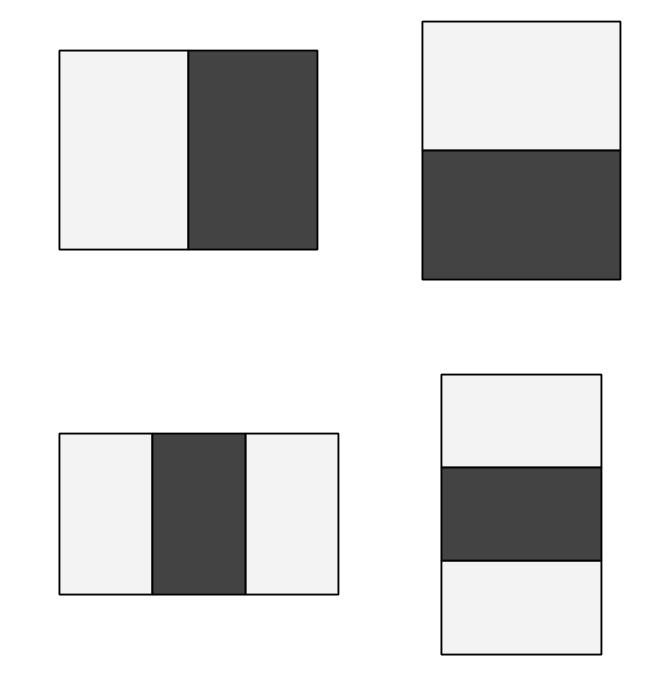
\includegraphics[width=5cm]{img/feature_types.jpg}
    \caption{Tipi di feature di Haar utilizzati in \cite{Zhu13}.}
    \label{fig:features_type}
\end{wrapfigure}

L'equazione \ref{eq:haar_feature_informal} fornisce una descrizione informale del funzionamento delle feature di Haar. Con $E(Area)$ si intende la somma delle intensità di tutti i pixel che appartengono all'area specificata.

\begin{equation}
    f(Img) = E(Area_{white}) - E(Area_{black})
    \label{eq:haar_feature_informal}
\end{equation}

Il segno del valore di una feature identifica il verso della variazione. Se si prende in esame la forma di feature in alto a sinistra della figura \ref{fig:features_type}, un valore positivo denota un'intensità mediamente maggiore nella regione bianca rispetto alla media della regione nera e viceveresa.

Evidenziare le variazioni di intensità delle immagini integrali attraverso l'applicazione delle feature di Haar equivale ad evidenziare le differenze di quota medie delle regioni individuate dalla feature e questo le rende particolarmente adatte a questa applicazione.

In seguito sarà necessario dover calcolare gruppi di feature in diverse scale. Ridimensionare un gruppo di feature è una cosa semplice e verrà trattata in seguito, ma affinchè il valore della feature sia il meno possibile sensibile ai ridimensionamenti è necessario rapportare tale valore all'estensione totale dell'area interessata (equazione \ref{eq:haar_scale_invariant}).

\begin{equation}
    f'(Img) = \frac{E(Area_{white}) - E(Area_{black})}{size(Area_{white}) + size(Area_{black})}
    \label{eq:haar_scale_invariant}
\end{equation}

\section{Dalle Wavelet di Haar alle Feature}
\label{sec:haar_wavelet}
Le feature di Haar derivano dall'estensione bidimensionale delle wavelet di Haar, che sono il primo esempio di wavelet e vennero sviluppate nel 1909 da Alfrèd Haar \cite{Haar10}.
La wavelet madre (equazione \ref{eq:mother_wavelet}) è una funzione oscillante di lunghezza finita, caratteristica comune a tutti i tipi di wavelet.

\begin{equation}
\label{eq:mother_wavelet}
    \psi(x) =
    \begin{cases}
        1 & 0 \leq t < 1/2 \\
        -1 & 1/2 \leq t < 1 \\
        0 & \text{ altrimenti }
    \end{cases}
\end{equation}

Ogni segnale può essere rappresentato per mezzo delle wavelet di Haar. Costituiscono un sistema di rappresentazione duale alla serie di Fourier.

\begin{figure}[!htb]
    \minipage{0.45\textwidth}
    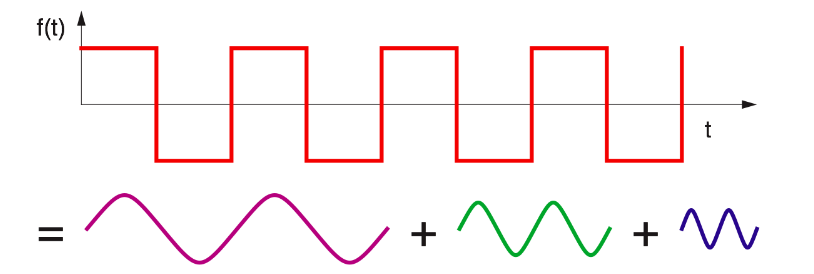
\includegraphics[width=\linewidth]{img/fourier_rapresentation.png}
    \caption{Rappresentazione di un segnale con una serie di funzioni armoniche.}
    \label{fig:awesome_image1}
    \endminipage\hfill
    \minipage{0.45\textwidth}
    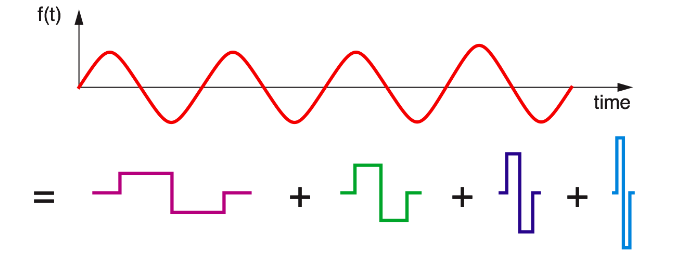
\includegraphics[width=\linewidth]{img/haar_rapresentation.png}
    \caption{Rappresentazione di un segnale con una serie di wavelet di Haar.}
    \label{fig:awesome_image2}
    \endminipage
\end{figure}

Alfrèd Haar propose anche la prima DWT (\emph{Discrete Wavelet Transform}) con la quale, le wavelet che compongono un segnale, vengono campionate discretamente.
Le applicazioni sono notevoli e ad ampio spettro, prime tra tutte quelle nell'ambito della codica dei segnali e nella compressione dei dati. Per fare un esempio, lo standard di compressione JPEG2000 sfrutta la trasformazione DWT \cite{Jpeg2000} per ottenere risultati qualitativamente migliori rispetto allo standard precedente.

Una variante della trasformazione DWT con le wavelet di Haar bidimesionali (figura \ref{sec:haar_wavelet}) è stata utilizzata da \citet{Oren97} in un sistema in grado di riconoscere la presenza di pedoni in delle immagini.

\begin{wrapfigure}{L}{0cm}
    \centering
    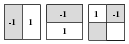
\includegraphics[width=3cm]{img/haar_wavelet.png}
    \caption{Wavelet di Haar bidimensionali utilizzate in \cite{Oren97}.}
    \label{fig:haar_wavelet}
\end{wrapfigure}

Applicando alle immagini la trasformata DWT in diverse scale, si passa da una rappresentazione dell'immagine in scala dei grigi, ad una rappresentazione in termini di coefficienti delle wavelet di Haar.
Tali coefficienti denotano le differenze di intensità tra le aree adiacenti dell'immagine e vengono utilizzati per evidenziare analogie strutturali delle immagini che contengono la figura di un pedone.

\begin{wrapfigure}{R}{0cm}
    \centering
    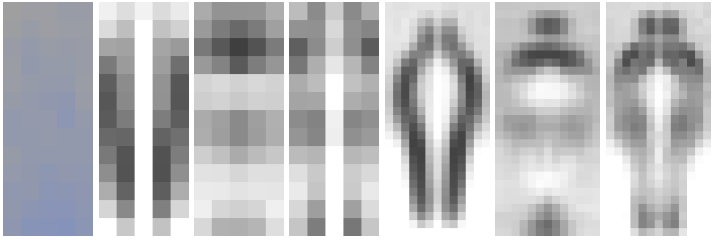
\includegraphics[width=8cm]{img/pedestrian_dwt.png}
    \caption{Coefficienti delle wavelet di trasformate DWT di diverse scale applicate alla stessa immagine. I coefficienti vengono codificati utilizzando la scala dei grigi \cite[Figura 3]{Oren97}.}
    \label{fig:non_standard_dwt}
\end{wrapfigure}

Nella descrizione di un framework generale per l'object detection, \citet{Papageorgiou98} utilizzano la trasformata DWT a wavelet di Haar bidimensionali non per l'estrazione di un template dell'oggetto espresso in variazioni di intensità, bensì per la selezione delle wavelet più significative al fine del riconoscimento dell'oggetto.

Una wavelet di Haar bidimensionale di una data dimensione, utilizzata per campionare un'immagine in una posizione specifica mette in evidenza le differenze di intensità dell'immagine nella regione descritta dall'area della wavelet. Tale differenza di intensità costituisce una proprietà osservabile e misurabile dell'immagine che ritrae l'oggetto. Queste sono le \emph{Haar-like feature} (o semplicemente feature di Haar).

\section{Immagine Integrale}
\label{sec:integral_image}
Le feature di Haar vengono utilizzate anche nel riconoscimento dei volti umani di Viola-Jones.
Sono molto apprezzate, sebbene siano molto primitive rispetto ad altri tipi più evoluti di feature, per la loro efficienza computazionale.

Il calcolo della somma delle intensità dei pixel di un'area è un'operazione il cui costo aumenta linearmente con la quantità di pixel. Introducendo il concetto di \emph{immagine integrale}, ottenuta rielaborando l'immagine di partenza, tale somma viene eseguita una volta per ogni immagine, permettendo in seguito di calcolare il valore di ogni feature in un tempo costante.

\begin{definition}
    Sia $I$ un'immagine larga $w$ pixel ed alta $h$ pixel. Con la scrittura $I(x, y)$ si identifica il pixel dell'immagine $I$ che si trova alla colonna $x$ e alla riga $y$.
    Si definisce \emph{immagine integrale} (altrimenti detta \emph{Summed Area Table}) una seconda immagine $SAT$ delle stesse dimensioni per cui vale $\forall x \in [1,w], y \in [1,h]$:
    \begin{equation}
        SAT(x, y) = \sum_{i = 1}^{x} \sum_{j = 1}^{y} I(i, j)
    \end{equation}
\end{definition}

\begin{wrapfigure}{L}{0cm}
    \centering
    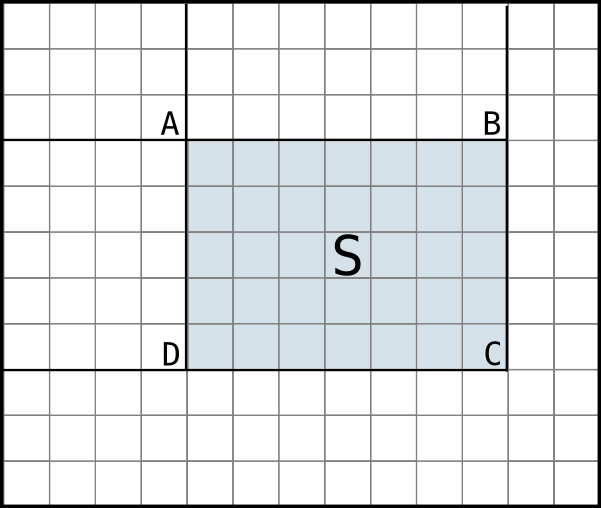
\includegraphics[width=5cm]{img/integral_image_sum.png}
    \caption{}
    \label{fig:integral_image_sum}
\end{wrapfigure}

Calcolare la somma del valore dei pixel contenuti in una regione rettangolare dell'immagine originale, con l'ausilio dell'immagine integrale, è un'operazione velocissima.

Si consideri la figura \ref{fig:integral_image_sum}: si vuole calcolare la somma del valore dei pixel nella regione $S$ evidenziata. I vertici del rettangolo saranno i punti $A:(x_1,y_1)$, $B:(x_2,y_1)$, $C:(x_2,y_2)$, $D:(x_1, y_2)$, notando che $1 \leq x_1 \leq x_2 \leq w$ e che $1 \leq y_1 \leq y2 \leq h$ \footnote{Nelle immagini raster, si iniziano a contare le colonne e le righe dal punto in alto a sinistra.}.
Quindi:

\begin{align*}
    \sum_{i = x_1}^{x_2} \sum_{j = y_1}^{y_2} I(i,j) =
    \sum_{i = 1}^{x_2} \sum_{j = y_1}^{y_2} I(i,j) - \sum_{i = 1}^{x_1} \sum_{j = y_1}^{y_2} I(i,j) = \\
    =
    \left(
    \sum_{i = 1}^{x_2} \sum_{j = 1}^{y_2} I(i,j) -
    \sum_{i = 1}^{x_2} \sum_{j = 1}^{y_1} I(i,j)
    \right)
    -
    \left(
    \sum_{i = 1}^{x_1} \sum_{j = 1}^{y_2} I(i,j) -
    \sum_{i = 1}^{x_1} \sum_{j = 1}^{y_1} I(i,j)
    \right) = \\
    = SAT(C) - SAT(B) - SAT(D) + SAT(A)
\end{align*}

Elaborare l'immagine integrale è un'operazione con complessità computazionale $\Theta(w \cdot h)$, cioè il cui costo varia linearmente con la dimensione dell'immagine. Una volta ottenuta però, permette di calcolare qualsiasi somma di pixel in regioni rettangolari con operazioni di complessità $\Theta(1)$.

Grazie all'immagine integrale è quindi possibile valutare in tempi brevi, gruppi enormi di feature sulla stessa immagine.


\section{Decision Stump}
\label{sec:decision_stump}
\begin{wrapfigure}{R}{0cm}
    \centering
    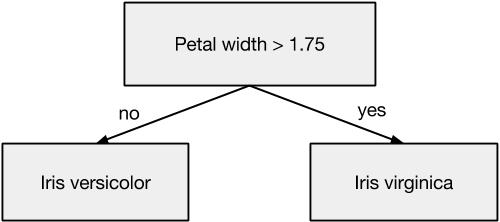
\includegraphics[width=7cm]{img/decision_stump.jpg}
    \caption{Esempio di decision stump usato per dividere gli oggetti in due classi delle tre descritte nel dataset delle caratteristiche dei fiori di Iris \cite{Fisher36}}
    \label{fig:decision_stump}
\end{wrapfigure}
Si tratta di \emph{alberi decisionali} binari di profondità unitaria.
Vi è un unico test alla radice, in base al quale si decide l'appartenenza di un oggetto ad due classi. Combinando tra loro diversi decision stump, è possibile creare alberi decisionali più complessi da poter utilizzare in alberi di classificazione non binari.

I decision stump costituiscono il meccanismo più semplice di classificazione che si può avere a disposizione. Il test da collocare alla radice dell'albero viene eseguito sul valore di una feature di Haar.

\begin{equation}
    test_1(x) =
    \begin{cases}
        true & \text{ se } f_1(x) < \theta_1\\
        false & \text{ altrimenti }
    \end{cases}
    \label{eq:decision_stump_minor}
\end{equation}

\begin{equation}
    test_2(x) =
    \begin{cases}
        true & \text{ se } f_2(x) > \theta_2\\
        false & \text{ altrimenti }
    \end{cases}
    \label{eq:decision_stump_maior}
\end{equation}

Le equazioni \ref{eq:decision_stump_minor} e \ref{eq:decision_stump_maior} descrivono due possibili test decisionali che possono essere collocati alla radice di un decision stump.
Per standardizzare la forma dei test si utilizzerà l'equazione \ref{eq:decision_stump}.

\begin{equation}
    test(x) =
    \begin{cases}
        true & \text{ se } f(x)p > p\theta\\
        false & \text{ altrimenti }
    \end{cases}
    \label{eq:decision_stump}
\end{equation}

In riferimento all'equazione \ref{eq:decision_stump}, $x$ è un'immagine di profondità, $f$ una feature di Haar ed $f(x)$ il valore della feature misurato sull'immagine $x$.
Il parametro $p \in \{ 1, -1 \}$, che assumerà il nome di \emph{polarità}, serve solamente per invertire il segno della disequazione all'occorrenza.
Il parametro $\theta$ è il valore di \emph{soglia} (\emph{threshold}).

Utilizzare i decision stump con le immagini di profondità equavale a verificare la presenza di variazioni di quota tra regioni contigue dell'immagine al di sopra o al di sotto di un certo valore di soglia.
La scelta del valore di soglia non è un problema banale e sarà trattato approfonditamente nel prossimo capitolo.

Il successo o l'insuccesso del test deve essere interpretato correttamente ai fini della classificazione. Di qui in avanti qualsiasi test decisionale applicato ad immagini di profondità che avrà successo, segnalerà la presenza di una persona, mentre, viceversa, quelli che non avranno successo ne segnaleranno l'assenza.
